% !TeX root = ../thesis.tex
% !TeX spellcheck = en_GB
% !TeX encoding = UTF-8

A forward start option is an option that starts at a specified future date (called the \emph{determination date}), with an expiration date set further in the future\footnote{\url{http://www.math.umn.edu/~spirn/5076/Lecture16.pdf} (Page 5)}. A forward start option starts at a specified date in the future; however, the premium is paid in advance, and the time of expiration is established at the time the forward start option is purchased. Since the asset price at the start of this option is not known a priori, it is common to specify that the strike price will be set in the future so that the option is initially at the money or a certain percentage in the money or out of the money.

The payoff of a forward start call option with time to expiration $ T $ and such that the strike is determined at the money at time $ u $ is given by $ (S_T - S_u)_+ $\footnote{\url{http://www.stat.nus.edu.sg/~stalimtw/MFE5010/PDF/L2forward.pdf}}

A \emph{cliquet option} or a \emph{ratchet option} is an exotic option consisting of a series of consecutive forward start options. The first such option is active immediately, and once it expires the second comes into existence, and so on. Each option is struck \emph{at-the-money} when it becomes active. Therefore, such an option periodically settles and resets its strike price at the level of the underlying during the time of settlement. Investors can opt to receive their payout either when each option expires or wait until the entire time has elapsed.

Usually, the return on a cliquet option is capped and floored. The capping and flooring may be local or global (or both). The motivation behind bounding the return is to provide the investor safety against downside risks, yet allowing significant upside potential. Consequently, the investor is also constrained from having unbounded gains. Capping the maximum ensures that the payoff is never too extreme and therefore that the value of the contract is not too outrageous. Some variants of cliquet options are as follows:
\begin{description}
	\item[Reverse cliquet] Amounts to a cash flow minus a capped cliquet of puts.
	\item[Digital cliquet] The forward-starting options are digital options.
\end{description}

The following example, copied verbatim from Investopedia\footnote{\url{http://www.investopedia.com/terms/c/cliquet.asp}}, provides a good illustration.
\begin{eg}
	A three-year cliquet option with a strike of 1000 would expire worthless on the first year if the underlying was to be 900. This value (900) would then be the new strike price for the following year and should the underlying on the settlement be 1200, the contract holder would receive a payout and the strike would reset to this new level. Higher volatility provides better conditions for investors to earn profits.
\end{eg}



\paragraph{Literature review}
The literature for pricing of cliquet options is primarily based on partial differential equations (PDE) techniques. Notable mentions include Wilmott's finite difference (FD) approach in a non-linear uncertain volatility model (UVM) in 2002 \cite{Wilmott2002}. Later in 2006, Windcliff et al.\cite{Windcliff2006} explored a variety of modelling alternatives, including jump diffusion models, local volatility and UVM models, again using finite differences methods. They compared the use of a running sum of returns formulation to an average return formulation. Methods for grid construction, interpolation of jump conditions, and application of boundary conditions were also compared.


\paragraph{Lattice method}
Gaudenzi \emph{et al}\cite{Gaudenzi2011} introduced a discrete method for pricing cliquet options in the Cox Ross Rubinstein model \cite{Cox1979} introduced in Chapter \ref{cha:models}. This singular points method is faster than the alternative lattice based approaches available, while retaining a fair bit of flexibility to handle varying volatilities and rates of interest. Most of the chapter is inspired by this paper.

The central idea of the method, as we saw in Chapter \ref{cha:asian}, is to give, at every monitoring date, a continuous representation of the cliquet option price as a piecewise-linear function of the sum of the returns over the corresponding period. This function is characterized only by a set of points, called \emph{singular points}, which can easily be computed recursively by backward induction. Although the number of singular points grows rapidly at every monitoring date, it is possible to reduce their number drastically in a
straightforward way, controlling the error involved by the elimination procedure at the same time. Moreover, the error control process leads automatically to the convergence of the approximations to the continuous value.



\section{Cliquet contracts and models}
\label{sec:clq-models}

Just as in the case of Asian options, we shall assume that the evolution of the prices of the risky asset $ (S_t)_t $ is governed by the Black-Scholes stochastic differential equation as discussed in Equation \ref{eq:continuous-risky-sde-risk-neutral} of Chapter \ref{cha:models}. Its solution is given by Equation \ref{eq:continous-risky}b. Whenever there is a continuous divident yield, we modify the equation according the remark \ref{rem:continuous-dividend}. Moreover, we shall consider the discrete model setup exactly as described in the beginning of Section \ref{sec:asian-binom} of Chapter \ref{cha:asian}.


Let $T$ be the maturity of the cliquet contract. Let the payoffs depend on the $ N $ preordained observation times $ t_1, t_2, \dots, t_{N} $ ($ t_0 = 0 $). At these observation times, the value of the underlying are $ ( S_i )_i, S_i = S_{t_i}, i \in \left[ N \right] $. The returns for the time interval $ ( t_{i-1}, t_i ] $ are given by
\begin{equation}
	\label{eq:clq-return}
	R_i = \frac{S_i - S_{i-1}}{S_{i-1}} = \frac{S_i}{S_{i-1}} - 1 \ .
\end{equation}

During each time interval, the return is capped and floored locally by the quantities $ C_{loc} $ and $ F_{loc} $. In other words, we consider the quantity $ \max \{ F_{loc}, \min \{ C_{loc}, R_i \} \} $ rather than the return itself. The sum of these quantities till time $t_i$ is called the `running sum' and is given by
\begin{equation}
	\label{eq:clq-rsz}
	Z_i = \sum_{k = 1}^{i} \max \{ F_{loc}, \min \{ C_{loc}, R_k \} \}.
\end{equation}

We also consider a global cap $ C_{glob} $ and floor $ F_{glob} $. Thus, the expression for the payoff finally becomes
\begin{equation}
	\label{eq:clq-rsz}
	\mathrm{payoff} = \mathrm{notional} \cdot \max \{ F_{glob}, \min \{ C_{glob}, Z_{N} \} \}.
\end{equation}

For ease of notation, we take $ \mathrm{notional} = 1 $.

We note that the case $ C_{glob} > N C_{loc} $ is equivalent to $ C_{glob} = N C_{loc} $. Similarly, the case $ F_{glob} < N F_{loc} $ is equivalent to $ F_{glob} = N F_{loc} $. In general, we may write the following.
\begin{subequations}
	\label{eq:clq-update-glob}
	\begin{align*}
		F_{glob} &= \max \{ N F_{loc}, F_{glob} \}  \\
		C_{glob} &= \min \{ N C_{loc}, C_{glob} \}
	\end{align*}
\end{subequations}

We assume that the difference between two observation times is constant and we denote by $m$ the number of steps of the binomial tree in every period (so that the total number of steps of the binomial tree is $ n = m N $).



\section{The singular points method for cliquet options}
\label{sec:clq-sp}

The binomial method may always be used to price any option, including path-dependent ones. The binomial method looks through all possible paths of the underlying in order to price the option. The number of possible paths are $ 2 ^ {m N} $. Thus, the method is inherently extremely computationally expensive due to the exponential dependence of the number of paths on $m$ and $ N $. The theoretical computational complexity is $ O( m^{N} ) $, as in \cite[Page 128]{Gaudenzi2011}.

A modification of the singular points method described in the previous chapter solves this problem for cliquet options by the process of approximation. The method of approximation selectively removes certain paths that would be normally considered, but which do not affect the result in a significant manner. This may be done by putting an \emph{a priori} error bound while removing points. The method turns out to be significantly faster and memory efficient compared to known binomial techniques. Moreover, its flexible is evinced by the fact that it is adaptable for varying interest rate and volatility in each observational period.

The price function in the cliquet case is not necessarily convex due to the presence of a global cap (see Figure \ref{fig:clq-maturity}), as opposed to the Asian case. Since the algorithm starts from maturity, it follows that we cannot assume convexity at any point of time. It was primarily the convexity of the price functions in the Asian case that allowed us to obtain simple upper and lower bounds of the exact binomial price. Nevertheless, in the case of cliquet options, the singular points approach still provides an efficient binomial framework, even in the absence of convexity of the price functions, as we shall see.

We redefine singular points to exclude the constraint of convexity. The reader is advised to keep in mind the ideas introduced in Section \ref{subsec:asian-notations} of Chapter \ref{cha:asian}.

\begin{dfn}[singular points and singular values]
	\label{def:clq-sp}
	Let $ P = (P_i)_{i \in [n]} = ( (x_i, y_i) )_{i \in [n]} $, $ n \in \mathbb{N} $ be a sequence of points such that $ a = x_0 < x_1 < \dots < x_{n-1} < x_n = b \forall i \in [n] $
	
	Let $ f:[a,b] \to [0, \infty) $ be the function obtained by linear interpolation of the points in $P$. The definition of $f$ ensures that the function is continuous and piecewise-linear.
	
	Then, the elements of $P$ are called \emph{singular points of $f$} and the abscissae $ \{ x_i \}_{i \in [n]} $ are called \emph{singular values of $f$}.
\end{dfn}


\begin{rem}[characterisation]
	\label{rem:clq-char}
	Note that the singular points characterise such a function completely, even without the requirement of convexity. This is clear from \ref{rem:asian-char}.
\end{rem}


\subsection{The method}
\label{subsec:clq-method}

Our aim is to look at every possible value taken by the running sum $Z$ within the bounds $ [ F_{loc}, C_{loc} ] $ for each time interval $ t_1, \dots, t_{N} $. If we know the price function at maturity, we may use a backward procedure (in time) in order to obtain a continuous representation of the cliquet price as a piecewise-linear function of the running sum $Z$. Since it is piecewise-linear and continuous, the function may be represented using its singular points. Thus, we see an evolution of singular points as we go back in time. Since the number of singular points may be significantly high for any computer, we shall introduce an error controlled approximation procedure to reduce the number of singular points.

Let the number of singular points at each observational time $ t_i $ be $ L_{i} $, where $ i \in \{ 1, \dots, N \} $. For each singular point $ l \in \{ 1, \dots, L_i \} $, the abscissa is called the \emph{singular running sum} $ Z_i^l $ and the ordinate is called the \emph{singular price} $ P_i^l $. Thus, the singular points are denoted by
\begin{equation*}
	( Z_i^l, P_i^l ) \qquad \forall l \in \{ 1, \dots, L_i \}
\end{equation*}


\paragraph{At maturity}
At maturity ($ t_{N{obs}} = T $), for every running sum $Z$, the price of the cliquet option $ V_{N}(Z) $ as function of $Z$, is given by
\begin{equation}
	\label{eq:clq-vnobs-maturity}
	V_{N}(Z) = \max \{ Fglob, \min\{ Cglob, Z \} \}
\end{equation}

We note the following.
\begin{enumerate}
	\item $ V_{N}(Z) $ is a continuous and piecewise-linear function 
	\item $ V_{N}(Z) $ is defined in the interval $ [ N F_{loc}, N C_{loc} ] $
	\item There are only four points where the function changes slope, namely $ N F_{loc} $, $ F_{glob} $, $ C_{glob} $ and $ N C_{loc} $. This is because if $ Z < F_{glob} $, the price is constant. Same can be said about $ Z > C_{glob} $. Thus the four numbers enumerated above form the complete set of singular running sums at maturity ($ L_N = 4 $).
\end{enumerate}

Focusing further on point 3 above, we note down the singular running sums and corresponding prices.
\begin{table}[h]
	\centering
	\caption{Singular points at maturity}
	\label{tab:clq-maturity}
	\begin{tabular}{ccc}
		\toprule
		$l$  &  $ Z_{N}^l $  &  $ P_{N}^l $ \\
		\midrule
		1  &  $ N F_{loc} $  &  $ F_{glob} $ \\
		2  &  $ F_{glob} $  &  $ F_{glob} $ \\
		3  &  $ C_{glob} $  &  $ C_{glob} $ \\
		4  &  $ N C_{loc} $  &  $ C_{glob} $ \\
		\bottomrule
	\end{tabular}
\end{table}

A more visual representation of the price function at maturity is given in Figure \ref{fig:clq-maturity}.
\begin{figure}[h]
	\centering
	
	\definecolor{cqcqcq}{rgb}{0.7529411764705882,0.7529411764705882,0.7529411764705882}
	\definecolor{xdxdff}{rgb}{0.49019607843137253,0.49019607843137253,1.}
	\definecolor{qqqqff}{rgb}{0.,0.,1.}
	\begin{tikzpicture}[line cap=round,line join=round,>=triangle 45,x=1.0cm,y=1.0cm]
	\draw[->,color=black] (0.,0.) -- (9.,0.);
	\foreach \x in {,1.,2.,3.,4.,5.,6.,7.,8.}
	\draw[shift={(\x,0)},color=black] (0pt,2pt) -- (0pt,-2pt);
	\draw[color=black] (8.77813297657717,0.054247335995569544) node [anchor=south west] { Z};
	\draw[->,color=black] (0.,0.) -- (0.,5.);
	\foreach \y in {,1.,2.,3.,4.}
	\draw[shift={(0,\y)},color=black] (2pt,0pt) -- (-2pt,0pt);
	\draw[color=black] (0.06780919373316127,4.698691618151926) node [anchor=west] { P};
	\clip(-0.5,-0.5) rectangle (9.,5.);
	\draw [line width=1.2pt] (1.,1.)-- (2.,1.);
	\draw [line width=1.2pt] (2.,1.)-- (7.,4.);
	\draw [line width=1.2pt] (7.,4.)-- (8.,4.);
	\draw [line width=0.4pt,color=cqcqcq] (1.,1.)-- (1.,0.);
	\draw [line width=0.4pt,color=cqcqcq] (2.,1.)-- (2.,0.);
	\draw [line width=0.4pt,color=cqcqcq] (7.,4.)-- (7.,0.);
	\draw [line width=0.4pt,color=cqcqcq] (8.,4.)-- (8.,0.);
	\draw [line width=0.4pt,color=cqcqcq] (1.,1.)-- (0.,1.);
	\draw [line width=0.4pt,color=cqcqcq] (7.,4.)-- (0.,4.);
	\begin{scriptsize}
	\draw [fill=qqqqff] (1.,1.) circle (1.5pt);
	\draw[color=qqqqff] (0.9258283422770954,1.3896041224221845) node {$S_1$};
	\draw [fill=qqqqff] (2.,1.) circle (1.5pt);
	\draw[color=qqqqff] (1.7666623445682952,1.3896041224221845) node {$S_2$};
	\draw [fill=qqqqff] (7.,4.) circle (1.5pt);
	\draw[color=qqqqff] (7.204959681967829,3.5594975622449665) node {$S_3$};
	\draw [fill=qqqqff] (8.,4.) circle (1.5pt);
	\draw[color=qqqqff] (8.181412071725351,3.6001830642416435) node {$S_4$};
	\draw [fill=xdxdff] (1.,0.) circle (1.5pt);
	\draw[color=xdxdff] (0.5732205348646567,-0.31918696143825614) node {$F_{loc} N$};
	\draw [fill=xdxdff] (2.,0.) circle (1.5pt);
	\draw[color=xdxdff] (2.254888539447056,-0.31918696143825614) node {$F_{glob}$};
	\draw [fill=xdxdff] (7.,0.) circle (1.5pt);
	\draw[color=xdxdff] (6.526867744636216,-0.31918696143825614) node {$C_{glob}$};
	\draw [fill=xdxdff] (8.,0.) circle (1.5pt);
	\draw[color=xdxdff] (8.452648846657995,-0.3463106294360409) node {$C_{loc} N$};
	\draw [fill=xdxdff] (0.,1.) circle (1.5pt);
	\draw[color=xdxdff] (-0.050624047480426926,0.73863609047535) node {$F_{glob}$};
	\draw [fill=xdxdff] (0.,4.) circle (1.5pt);
	\draw[color=xdxdff] (-0.07774772497369145,3.7358014042305676) node {$C_{glob}$};
	\end{scriptsize}
	\end{tikzpicture}
	
	\caption{The price function at maturity}
	\label{fig:clq-maturity}
\end{figure}


\paragraph{The penultimate time step}

We consider the time step $ N - 1 $. If the running sum at time $ t_{N - 1} $ is denoted by $ Z $, then the corresponding price depends on the possible returns of the underlying asset during the time interval $ [ t_{N - 1}, T ] $.

We revisit equation \ref{eq:clq-return} once more. Now we note that since the number of time steps in each interval is $m$, there will be $m$ up movements or down movements of the asset. Thus, there are $ m + 1 $ possible outcomes, given by $ S_i = u^{-m + 2j} S_{i-1}, j \in [m] $. Corresponding to these cases, there are also $ m + 1 $ returns, given by
\begin{equation}
	\label{eq:clq-return-final}
	R_j = u^{-m + 2j} - 1 \qquad j \in [m]
\end{equation}

Since the probability of an up movement in time $ \Delta T $ is $p$, we have that the probability of each return is distributed binomially, and is given by
\begin{equation}
	\label{eq:clq-prb-binom}
	p_j = \binom{m}{j} p^j (1-p)^{m-j}
\end{equation}

The above derivations assume that there has been no local flooring or capping of the returns. In the case of such bounds, the actual possibilities are fewer in number, and we need to put bounds on $j$. We can do this in the following fashion.

In the case of a local floor, we must have
\begin{alignat*}{9}
	                 &&  F_{loc}  \quad & \ge \quad  u^{ -m + 2 j_{\min} } - 1 && \\
	\implies  \qquad &&  \log(F_{loc} + 1)  \quad & \ge \quad  ( -m + 2 j_{\min} ) \log(u)  &&  \qquad \qquad \dots (\log \text{is monotonic}) \\
	\implies  \qquad &&  \frac{\log(F_{loc} + 1)}{\log(u)}  \quad & \ge \quad  ( -m + 2 j_{\min} )  &&  \qquad \qquad \dots (u > 1 \implies \log(u) > 0) \\
	\implies  \qquad &&  j_{\min}  \quad & \le \quad  \frac{ \log(F_{loc} + 1) }{ 2 \sigma \Delta T } + \frac{m}{2}  &&  \qquad \qquad \dots (u = e^{ \sigma \Delta T }) \\
	\implies  \qquad &&  j_{\min}  \quad & = \quad  \floor{ \frac{ \log(F_{loc} + 1) }{ 2 \sigma \Delta T } + \frac{m}{2} }  &&  \qquad \qquad \dots (j \in [m]) \\
\end{alignat*}
Where $ \floor{\cdot} $ denotes the floor function.

Similarly, in the case of local cap, we have
\begin{alignat*}{9}
	                 &&  C_{loc}  \quad & \le \quad  u^{ -m + 2 j_{\max} } - 1 && \\
	\implies \qquad  &&  \log(C_{loc} + 1)  \quad & \le \quad  ( -m + 2 j_{\max} ) \log(u)  &&  \qquad \qquad \dots (\log \text{is monotonic}) \\
	\implies \qquad  &&  \frac{\log(C_{loc} + 1)}{\log(u)}  \quad & \le \quad  ( -m + 2 j_{\max} )  &&  \qquad \qquad \dots (u > 1 \implies \log(u) > 0) \\
	\implies \qquad  &&  j_{\max}  \quad & \ge \quad  \frac{ \log(C_{loc} + 1) }{ 2 \sigma \Delta T } + \frac{m}{2}  &&  \qquad \qquad \dots (u = e^{ \sigma \Delta T }) \\
	\implies \qquad  &&  j_{\max}  \quad & = \quad  \ceil{ \frac{ \log(C_{loc} + 1) }{ 2 \sigma \Delta T } + \frac{m}{2} }  &&  \qquad \qquad \dots (j \in [m]) \\
\end{alignat*}
Where $ \ceil{\cdot} $ denotes the ceiling function.

We represent by $ j_0 $ the number of possibilities of the return after enforcing the local floor and cap. Summarising
\begin{subequations}
	\label{eq:clq-j-mix-max}
	\begin{align}
		j_{\min} &= \floor{ \frac{ \log(F_{loc} + 1) }{ 2 \sigma \Delta T } + \frac{m}{2} }  \\
		j_{\max} &= \ceil { \frac{ \log(C_{loc} + 1) }{ 2 \sigma \Delta T } + \frac{m}{2} }  \\
		j_0 &= j_{\max} - j_{\min}
	\end{align}
\end{subequations}

$ \forall j \le j_{\min} $, the return is $ F_{loc} $, and $ \forall j \ge j_{\max} $, the return is $ C_{loc} $. For the other indices, the return remains unchanged.

We shift the indices from $ \{ j_{\min}, \dots, j_{\max} \} $ to $ \{ 0, \dots, j_0 \} $ by putting $ j' = j - j_{\min} $. Table \ref{tab:clq-shift} highlights the shifted indices, and the corresponding returns and probabilities.
\begin{table}[h]
	\centering
	\caption{Shifted returns and probabilities}
	\label{tab:clq-shift}
	\begin{tabular}{cccc}
		\toprule
		Range$(j)$  &  $ j' $  &  $ R_j' $  &  $ p_j' $  \\
		\midrule
		$ j \le j_{\min} $  &  $ 0 $  &  $ F_{loc} $  &  $ \sum_{k=0}^{j_{\min}} p_k $  \\
		$ \{ j_{\min} + 1, \dots, j_{\max} - 1 \} $  &  $ j - j_{\min} $ &  $ R_{j + j_{\min}} $  &  $ p_{j + j_{\min}} $  \\
		$ j \ge j_{\max} $  &  $ j_0 $  &  $ C_{loc} $  &  $ \sum_{k=j_{\max}}^{m} p_k $  \\
		\bottomrule
	\end{tabular}
\end{table}

\begin{rem}[shifted indices]
	\label{rem:clq-shift}
	Note that the $ j' $s represents the indices of the possible paths that can \emph{actually} be taken respecting the constraints of the local floor and cap, whereas $ j $ represents the indices of all possible paths without respect to any constraints. Thus, we are more interested in the shifted indices. Similarly, $ p_j' $ represents the probability of taking the path $ j' $, and $ R_j' $ represents the corresponding return.
\end{rem}

Now we focus on how to determine the price function at time $ t_{N - 1} $. Recall that at maturity, the function $ V_{N}(Z) $ giving the price of the cliquet option as a function of the running sum $ Z $ at maturity, is the piecewise linear function whose singular points are presented in Table \ref{tab:clq-maturity}. At the penultimate time step $ t_{N - 1} $, we must have $ Z \in [ (N-1) F_{loc}, (N-1) C_{loc} ] $. Note that $ Z $ is the running sum till the penultimate time step. The price function at this time is given as a discounted conditional expectation of the price function at maturity given the information at penultimate time. Thus
\begin{equation}
	\label{eq:clq-penultimate}
	V_{N-1} (Z) = e^{- m \Delta T} \sum_{j=0}^{j_0} \left[ p_j' V_{N} (Z + R_j') \right] ,
\end{equation}
where $ p_j' $ and $ R_j' $ are given in Table \ref{tab:clq-shift}.

Since $ V_{N} $ is piecewise-linear and continuous, and the above is just a linear combination of such functions, the resulting function is also piecewise-linear and continuous, and thus may be completely represented by singular points. The next logical step is of course to figure out a method to compute these singular points.

From equation \ref{eq:clq-penultimate}, we note that each singular point $ l $ at maturity may have $ j_0 + 1 $ possible returns, given by
\begin{equation}
	\label{eq:clq-b}
	B_{l,j} = Z_N^l - R_j' \qquad j \in [j_0]
\end{equation}

Then the maximum number of singular points at time $ t_{N-1} $ is $ ( j_0 + 1 ) L_N $. But not all the running sums at time $ t_{N-1} $ would belong to the interval $ [ (N-1) F_{loc}, (N-1) C_{loc} $. All the $ B_{l,j} $ which belong to the interval become the abscissa of a singular point at time $ t_{N-1} $. The corresponding singular price is determined by formula \ref{eq:clq-penultimate}. The term $ V_{N} (B_{l,j} + R_k') $, required by the formula, is computed using linearity of the price function at maturity. We just need to figure out the interval $ l_0 $ such that $ ( B_{l,j} + R_k' ) \in [ Z_N^{l_0}, Z_N^{l_0 + 1} ] $, and evaluate $ V_{N} (B_{l,j} + R_k') $ by linear interpolation of the extrema. Such an interpolation gives not an approximation by the exact value due to the piecewise-linear nature of the original function.

Finally, the singular points thus obtained are sorted in ascending order on the basis of the running sums. This ordered sequence of singular points $ ( ( Z_{N-1}^l, P_{N-1}^l ) )_l , l \in \{ 1, \dots, L_{N-1} \} $ completely characterises the price function at time $ V_{N-1}(Z) $.


\paragraph{At all times}
The previous argument may be applied iteratively in a backward fashion at each step $ N-2, N-3, \dots, 1, 0 $ to obtain the singular points at each time step. At time 0, there is only one singular point $ (0, P_0^1) $, and $ P_0^1 $ provides the exact binomial price of the cliquet option. The equality of this price and the exact binomial price is proved in Proposition \ref{thm:clq-equality}.


\begin{prp}[The singular points method gives the binomial price]
	\label{thm:clq-equality}
	$ P_0^l $ coincides with the exact binomial price with $ n $ time steps of the cliquet option.
\end{prp}

\begin{proof}
	Let the running sum $ Z_{i_1, \dots, i_k} = \sum_{j=1}^{k} R_{i_j}', \  (i_1, \dots, i_k) \in [j_0]^k, k \in \{ 1, \dots, N \} $, and associate them to the prices $ P_{i_1, \dots, i_k} $.
	Then the exact binomial price $ Q_n $ of the cliquet option is given by
	\begin{equation*}
		Q_n = e^{-rT} \sum_{i_1, \dots, i_N = 0}^{j_0} \left( p_{i_1}' \cdot \dots \cdot p_{i_N}' \max \left\{ F_{glob}, \min \left\{ C_{glob}, Z_{i_1, \dots, i_N} \right\} \right\} \right) ,
	\end{equation*}
	where $ p_{i_k}' $ is the probability of actually taking the path $ i_k $ at the time interval $ k $. This expression can be computed backward.
	
	At maturity, set $ P_{i_1, \dots, i_N} = \max \left\{ F_{glob}, \min \left\{ C_{glob}, Z_{i_1, \dots, i_N} \right\} \right\} $.
	
	Along the tree the prices $ P_{i_1, \dots, i_k}, k \in [N-1] $, are evaluated by the
	backward formula
	\begin{equation*}
		P_{i_1, \dots, i_k}  =  e^{-r \frac{T}{N}}  \sum_{j=0}^{j_0} p_j' P_{i_1, \dots, i_k, j}
	\end{equation*}
	
	Finally, we get $ Q_n = e^{-r \frac{T}{N}}  \sum_{j=0}^{j_0} p_j' P_j $.
	
	We now prove the result by backward induction. At maturity, for every choice of the running sum $ Z = Z_{i_1, \dots, i_N} $, the price $ P_{i_1, \dots, i_N} $ coincides with the value of the option $ v_N(Z) $. By construction (Equation \ref{eq:clq-penultimate}), this holds true
	also for every running sum evaluated at step $ N - 1 $, and iteratively, at all the nodes
	of the tree. Thus, the price $ Q_n $ coincides with the price $ P_0^1 $ determined by the singular points algorithm.
\end{proof}


\begin{rem}[Generalisation]
	The method is easily generalised to cases with (discrete) time-varying interest rates and volatilities. In other words, for each \emph{observed} time interval $ [t_{i-1}, t_{i}] $ denoted by $ i \in \{1, 2, \dots, N \} $, we can take different values of $ r_i, \sigma_i $. The technique requires modification only for the computation of the probabilities $ p' $ and the returns $ R' $ which have to be evaluated at every observation time by using the corresponding $ r_i $ and $ \sigma_i $.
	
	In fact, we may even take varying local floors and caps, denoted $ F_i^{loc}, C_i^{loc} $. In this case, we also have to compute $ j_{\min}, j_{\max}, j_0 $ for each period individually.
\end{rem}


\begin{rem}[Computational dependence on volatility]
	The time of computation of the pure binomial method for cliquet options is strongly dependent on the volatility. In fact the total number of paths needed to determine the price is $ m^N $. Because of the presence of the global cap and floor, the number of paths can be reduced to $ ( j_0 + 1 ) N $, where $ j_0 = j_{\max} - j_{\min} $. But $ j_0 $ is strictly dependent on $ \sigma $ (see Equation \ref{eq:clq-j-mix-max}) and the difference in the computational time between large and small volatilities becomes very high (see also Table \ref{tab:clq-results}).
\end{rem}



\subsection{Approximation}
\label{subsec:clq-approx}

The method demonstrated in Section \ref{subsec:clq-method} gives us the actual binomial price of the cliquet option. But as was mentioned earlier, the computational complexity of the method is theoretically the same as that of the binomial method, which is $ m^N $. But contrary to the binomial method, the singular point method enables us to use precise, efficient and controlled approximation to accelerate the procedure significantly. Thus its efficacy become apparent when we have time and memory constraints, or we wish to substantially increase the number of intermediate time steps.

The prime idea of the approximation procedure is to remove singular points in a controlled manner in order to simplify the computations. To this end, we fix a given maximal level $ h > 0 $ of the error in each period. Now, we eliminate singular points in a fashion so that the function after deletion of the points ($ \tilde{V}_i $) is different from the original function by less than ($ h $) at each point. This may be achieved as follows.

Start with the point $ ( Z_i^1, P_i^1 ) $. Find the largest index $ l > 1 $ such that the distances between the straight line joining $ ( Z_i^1, P_i^1 ) $ and $ ( Z_i^l, P_i^l ) $ and the points $ ( Z_i^2, P_i^2 ), ( Z_i^3, P_i^3 ), \dots, ( Z_i^{l-1}, P_i^{l-1} ) $ are always less than $ h $. Note that this, coupled with the fact that the original function is piecewise-linear, ensures that the differences in the values of the functions for any value of the running sum would be bounded over by $ h $. Now delete the points $ ( Z_i^2, P_i^2 ), ( Z_i^3, P_i^3 ), \dots, ( Z_i^{l-1}, P_i^{l-1} ) $. The point $ ( Z_i^l, P_i^l ) $ now becomes the second singular point, and we continue the procedure iteratively starting with this point till we cover all the points. Figure \ref{fig:clq-approx} elaborates on this graphically. The elimination of points $ S_3 $ to $ S_6 $ gives function $ V_1 $ (bold, blue), which has maximum error $ \le h $. Elimination of points $ S_3 $ to $ S_7 $ gives function $ V_2 $ (dashed, red), which has maximum error $ > h $. Thus we choose $ V_1 $ as the approximation function.

Since at each $ N $ the upper bound for the error is $ h $, if we repeat the approximation procedure at every observational time, the total error infused in the price of the option is bounded by $ Nh $.


\begin{figure}[h]
	\centering
	
	\definecolor{ffqqqq}{rgb}{1.,0.,0.}
	\definecolor{cqcqcq}{rgb}{0.7529411764705882,0.7529411764705882,0.7529411764705882}
	\definecolor{xdxdff}{rgb}{0.49019607843137253,0.49019607843137253,1.}
	\definecolor{qqqqff}{rgb}{0.,0.,1.}
	\begin{tikzpicture}[line cap=round,line join=round,>=triangle 45,x=1.0cm,y=1.0cm]
	\draw[->,color=black] (0.,0.) -- (12.,0.);
	\foreach \x in {,1.,2.,3.,4.,5.,6.,7.,8.,9.,10.,11.}
	\draw[shift={(\x,0)},color=black] (0pt,2pt) -- (0pt,-2pt);
	\draw[color=black] (11.72949725895975,0.0665249798016828) node [anchor=south west] { Z};
	\draw[->,color=black] (0.,0.) -- (0.,8.);
	\foreach \y in {,1.,2.,3.,4.,5.,6.,7.}
	\draw[shift={(0,\y)},color=black] (2pt,0pt) -- (-2pt,0pt);
	\draw[color=black] (0.08315626418944566,7.641135707448683) node [anchor=west] { P};
	\clip(-0.5,-0.5) rectangle (12.,8.);
	\draw [line width=2.pt,color=qqqqff] (1.,1.)-- (2.,1.);
	\draw [line width=1.2pt] (2.,1.)-- (3.,1.75);
	\draw [line width=1.2pt] (3.,1.75)-- (4.,2.);
	\draw [color=cqcqcq] (1.,1.)-- (1.,0.);
	\draw [color=cqcqcq] (2.,1.)-- (2.,0.);
	\draw [color=cqcqcq] (3.,1.75)-- (3.,0.);
	\draw [color=cqcqcq] (4.,2.)-- (4.,0.);
	\draw [color=cqcqcq] (1.,1.)-- (0.,1.);
	\draw [line width=1.2pt] (4.,2.)-- (6.,2.75);
	\draw [line width=1.2pt] (8.,4.)-- (9.,5.);
	\draw [line width=2.pt,color=qqqqff] (9.,5.)-- (10.,7.);
	\draw [color=cqcqcq] (6.,2.75)-- (6.,0.);
	\draw [color=cqcqcq] (9.,5.)-- (9.,0.);
	\draw [color=cqcqcq] (11.,7.)-- (11.,0.);
	\draw [line width=1.2pt] (6.,2.75)-- (8.,4.);
	\draw [color=cqcqcq] (8.,4.)-- (8.,0.);
	\draw [color=cqcqcq] (10.,7.)-- (10.,0.);
	\draw [line width=2.pt,color=qqqqff] (10.,7.)-- (11.,7.);
	\draw [line width=2.pt,color=qqqqff] (2.,1.)-- (9.,5.);
	\draw [line width=1.2pt,dash pattern=on 4pt off 4pt,color=ffqqqq] (2.,1.)-- (10.,7.);
	\draw [line width=1.6pt,dotted,color=qqqqff] (6.004094596374262,3.288054055071007)-- (6.,2.75);
	\draw [color=cqcqcq] (10.,7.)-- (0.,7.);
	\draw [line width=1.6pt,dotted,color=ffqqqq] (7.999695997451529,5.499771998088647)-- (8.,4.);
	\begin{scriptsize}
	\draw [fill=qqqqff] (1.,1.) circle (1.5pt);
	\draw[color=qqqqff] (0.9857079256833694,1.3545251161896577) node {$S_1$};
	\draw [fill=qqqqff] (2.,1.) circle (1.5pt);
	\draw[color=qqqqff] (1.8339018204157151,1.40441885104092) node {$S_2$};
	\draw [fill=qqqqff] (3.,1.75) circle (1.5pt);
	\draw[color=qqqqff] (2.9149332548785085,2.0530374041073274) node {$S_3$};
	\draw [fill=qqqqff] (4.,2.) circle (1.5pt);
	\draw[color=qqqqff] (4.21217097623386,1.8201999748014375) node {$S_4$};
	\draw [fill=xdxdff] (1.,0.) circle (1.5pt);
	\draw[color=xdxdff] (0.9191829143318129,-0.3917556036045157) node {$Z_1$};
	\draw [fill=xdxdff] (2.,0.) circle (1.5pt);
	\draw[color=xdxdff] (1.950320590280939,-0.35849311370367437) node {$Z_2$};
	\draw [fill=xdxdff] (3.,0.) circle (1.5pt);
	\draw[color=xdxdff] (2.948195760554287,-0.35849311370367437) node {$Z_3$};
	\draw [fill=xdxdff] (4.,0.) circle (1.5pt);
	\draw[color=xdxdff] (3.9294396779897456,-0.3917556036045157) node {$Z_4$};
	\draw [fill=xdxdff] (0.,1.) circle (1.5pt);
	\draw[color=xdxdff] (0.05435776676157797,0.8888502575778783) node {$F_{glob}$};
	\draw [fill=xdxdff] (0.,7.) circle (1.5pt);
	\draw[color=xdxdff] (0.021095261085799705,6.8262047048780685) node {$C_{glob}$};
	\draw [fill=qqqqff] (6.,2.75) circle (1.5pt);
	\draw[color=qqqqff] (6.1413963054290015,2.5519747526199485) node {$S_5$};
	\draw [fill=qqqqff] (8.,4.) circle (1.5pt);
	\draw[color=qqqqff] (8.153777898813587,3.8159493688519217) node {$S_6$};
	\draw [fill=qqqqff] (9.,5.) circle (1.5pt);
	\draw[color=qqqqff] (9.201546827600602,4.847086555778005) node {$S_7$};
	\draw [fill=qqqqff] (10.,7.) circle (1.5pt);
	\draw[color=qqqqff] (10.16615949219817,6.809573459927647) node {$S_8$};
	\draw [fill=qqqqff] (11.,7.) circle (1.5pt);
	\draw[color=qqqqff] (11.197297168147298,6.792942214977227) node {$S_9$};
	\draw [fill=xdxdff] (6.,0.) circle (1.5pt);
	\draw[color=xdxdff] (5.95845252421222,-0.3418618687532536) node {$Z_5$};
	\draw [fill=xdxdff] (8.,0.) circle (1.5pt);
	\draw[color=xdxdff] (7.954202864758916,-0.35849311370367437) node {$Z_6$};
	\draw [fill=xdxdff] (9.,0.) circle (1.5pt);
	\draw[color=xdxdff] (8.952078035032265,-0.37512435865409505) node {$Z_7$};
	\draw [fill=xdxdff] (11.,0.) circle (1.5pt);
	\draw[color=xdxdff] (10.897934617065292,-0.37512435865409505) node {$Z_9$};
	\draw [fill=xdxdff] (10.,0.) circle (1.5pt);
	\draw[color=xdxdff] (9.933321952467724,-0.35849311370367437) node {$Z_8$};
	\draw[color=qqqqff] (6.607071384889897,3.849211858752763) node {$V_1$};
	\draw[color=ffqqqq] (5.675721225968106,3.9822618183561285) node {$V_2$};
	\draw [color=qqqqff] (6.004094596374262,3.288054055071007)-- ++(-1.5pt,-1.5pt) -- ++(3.0pt,3.0pt) ++(-3.0pt,0) -- ++(3.0pt,-3.0pt);
	\draw[color=qqqqff] (6.340971339483671,3.0841745910334106) node {$\le$ h};
	\draw [color=ffqqqq] (7.999695997451529,5.499771998088647)-- ++(-1.5pt,-1.5pt) -- ++(3.0pt,3.0pt) ++(-3.0pt,0) -- ++(3.0pt,-3.0pt);
	\draw[color=ffqqqq] (8.30345917435459,4.847086555778005) node {>h};
	\end{scriptsize}
	\end{tikzpicture}
	
	\caption{Approximation procedure}
	\label{fig:clq-approx}
\end{figure}


\begin{rem}[Comparison with Asian options]
	While using approximations for Asian options, the error bound was $ nh $, where $ n $ was the number of time steps considered for computation (refer to Section \ref{sec:asian-approx} of Chapter \ref{cha:asian}). But in the case of the cliquet options, the error depends only on the $ h $ and the number of observations - precluding any dependence on the computational parameters. This technique gives a precise approximation of the price without considering upper and lower estimates.
\end{rem}

The following proposition proves that the approximation of the price obtained by this method does converge to the price of the cliquet option in the continuous model. The proposition and proof is directly from .


\begin{prp}[Convergence to the continuous model]
	\label{thm:convergence-continuous}
	Let us denote by $ Q_n^h $ the approximation of the price evaluated with $ n $ time steps and with maximal level of error at every monitoring date $ h = h(n) $. If $ h(n) \to 0 $ as $ n \to \infty $, then $ Q_n^{h(n)} $ converges to the price of the cliquet option in the continuous model.
\end{prp}

We skip the proof of the proposition since it is not the main focus of our exposition. The proof is mathematically delicate, and needs a general result on the weak convergence of stochastic processes. This is a generalisation of what we saw in Section \ref{subsec:discrete-to-continuous} of Chapter \ref{cha:models}. The result may be found in \cite{kushner1984approximation} and \cite{Kushner:1992:NMS:151172}, and we refer the interested reader to \cite[Proposition 2]{Gaudenzi2011} for a rigorous proof.



\clearpage
\section{The program}
\label{sec:clq-program}

\subsection{Algorithm}

\begin{algorithm}[H]
	\DontPrintSemicolon
	
	\KwIn{\\
		\qquad \emph{Contract details}  \\
		\qquad \quad time to maturity: $ T $ \\
		\qquad \quad number of observations: $ N $ \\
		\qquad \quad local floor and cap: $ F_{loc}, C_{loc} $  \\
		\qquad \quad global floor and cap: $ F_{glob}, C_{glob} $ \\
		
		\qquad \emph{Details of the underlying asset}  \\
		\qquad \quad initial price: $ s_0 $, volatility: $ \sigma $, continuous dividend rate: $ q $  \\
		
		\qquad \emph{Market parameters} -- spot interest rate: $ r $ \\
		
		\qquad \emph{Computational parameters} -- time steps within each observed period: $ m $ \\
	}
	
	\KwOut{The price of the option at the initial time}
	
	\Begin{
		Update $ F_{glob} $ and $ C_{glob} $ using Equations \ref{eq:clq-update-glob}. \;
		
		Set $ \Delta T, u, p $ from the formulae in Section \ref{sec:clq-models}. \;
		
		Compute the returns and probabilities using Equation \ref{eq:clq-return-final} and Equation \ref{eq:clq-prb-binom}. \;
		
		Compute $ j_{\min}, j_{\max}, j_0 $ (Equations \ref{eq:clq-j-mix-max}) and shifted returns (Table \ref{tab:clq-shift}). \;
		
		\tcp{$ S_i $ and $ S_+ $ denotes the current ($ i^{\mathrm{th}} $) and next ($ (i+1)^{\mathrm{th}} $) list of singular points.}
		
		$ S_N \leftarrow \{ (N F_{loc}, F_{glob}), (F_{glob}, F_{glob}), (C_{glob}, C_{glob}), (N C_{loc}, C_{glob}) \} $ \tcp{Table \ref{tab:clq-maturity}.}
				
		$ S_+ \leftarrow S_N $ \;
		
		\For{$ i \in \{ N-1, \dots, 0 \} $}{
			$ S_i \leftarrow \emptyset, \qquad L_+ \leftarrow \mathrm{length}(S_+) $ \;
			
			\ForAll{$ (l, j) \in [L_+] \times [j_0 + 1] $}{
				Compute $ B_{l,j} $ using Equation \ref{eq:clq-b}, replacing $ N $ by $ i $. \;
				
				\If{ $ ( B_{l,j} + R_k' ) \notin [ Z_N^{l_0}, Z_N^{l_0 + 1} ] $ } {
					Continue \tcp*{to the next item in the loop}
				}
				
				Find $ l_0 $ such that $ ( B_{l,j} + R_k' ) \in [ Z_{i+1}^{l_0}, Z_{i+1}^{l_0 + 1} ] $. \;
				
				Evaluate $ V_{i+1} (B_{l,j} + R_k') $ by linear interpolation of the extrema. \;
				
				Evaluate $ V_{i}(B_{l,j}) $ by using Equation \ref{eq:clq-penultimate}, replacing $ N $ by $ i $. \;
				
				$ S_i \leftarrow S_i \cup (B_{l,j}, V_{N-1}(B_{l,j})) $ \;
			}
			
			Approximate as described in Section \ref{subsec:clq-approx}. \;
			
			$ S_+ \leftarrow S_i $ \;
		}
		\KwRet{$ (S_i)_{1,2} $    \tcp*{Singular price at time 0} }
	}
	
	\caption{Pricing cliquet options using the singular points method}
\end{algorithm}


\clearpage
\subsection{Implementation}
The algorithm was implemented in Python 3.5.0 (2015-09-13).

\paragraph{mymath.py}
This file contains the $ \binom{n}{k} $ function.

\inputminted[tabsize=4]{python}{../code/mymath.py}
\label{lst:mymath}

\paragraph{cliquet.py}
This file contains the function \emph{cliquet\_sp}, which returns the price of the cliquet option at time 0.

\inputminted[tabsize=4]{python}{../code/cliquet.py}
\label{lst:clq}



\clearpage
\section{Results and conclusions}
\label{sec:clq-results}

In this section, we provide some numerical results that we have obtained from our program, along with the reported values of the same from \cite[Section 4]{Gaudenzi2011}. They compare the results with other techniques, namely Monte Carlo and the finite difference method of Windcliff et al\cite{Windcliff2006}. In all the experiments, the number of time steps considered were 10, 20, 50, 100, 200, 500 and 1000. The cases considered are as follows:
\begin{enumerate}
	\item Constant volatility of $ \sigma = 0.2 $
	\item Constant volatility of $ \sigma = 0.02 $, in order to test the efficiency of the methods for low volatility cases
	\item Varying volatility for each observational period, as $ \sigma(i) = 0.05 + 0.04i, i = 1, \dots, 8 $. (This is denoted by \emph{Var} in the $ \sigma $ column of Table \ref{tab:clq-results}.) The contract maturity is of 2 years, with quarterly monitoring dates.
\end{enumerate}
In order to obtain corroboration with the continuous value, we also report the price obtained by using Monte Carlo method with 1,000,000 of trials, along with the values in the 95\% confidence interval.

The specifications of the cliquet contract for the cases with constant volatility are as follows.
\begin{itemize}
	\item $ F_{loc} = 0, C_{loc} = 0.08, F_{glob} = 0.16, C_{glob} = \infty $
	\item $ T = 5 $ years
	\item $ N = 5 $
	\item $ r = 0.03 $
\end{itemize}

All simulations were run on a computer with the specifications given in Table \ref{tab:specs} of Chapter \ref{cha:asian}. All times were measured to 3 significant digits in seconds using the \emph{timeit} module of python, run from the terminal.

Table \ref{tab:clq-results} highlights the results.
\begin{table}[h]
	\centering
	\caption{Results for cliquet options}
	\label{tab:clq-results}
	%	\rowcolors{1}{Burlywood1}{}
	\begin{tabular}{rrccccc}
		\toprule
		\multirow{2}{1em}{$ \sigma $}  &  \multirow{2}{1em}{$ m $}
		&  \multicolumn{3}{c}{Price}  &  \multicolumn{2}{c}{Time (s)\tablefootnote{$ \infty $ means time taken is more than an hour.}}  \\
		\cmidrule(lr){3-5}\cmidrule(lr){6-7}
		&&  Bin  &  SP  &  MC  &  Bin  &  SP  \\
		\midrule
		\multirow{7}{2em}{$ 0.2 $}
		&    10  &  0.165661911  &  0.165661911  &  \multirow{7}{5em}{0.174106 (0.17398 -- 0.17423)}  &  0.000561  &  0.000555  \\
		&    20  &  0.172300056  &  0.172300056  &    &  0.000671  &  0.000675  \\
		&    50  &  0.172501269  &  0.172501269  &    &  0.00185  &  0.00175  \\
		&   100  &  0.172501269  &  0.173927464  &    &  0.00413  &  0.00297  \\
		&   200  &  0.173716366  &  0.173716366  &    &  0.0165  &  0.00828  \\
		&   500  &  0.173922597  &  0.173922671  &    &  0.0875  &  0.0437  \\
		&  1000  &  0.174051949  &  0.174051983  &    &  2.38  &  0.183  \\
		\midrule
		\multirow{7}{2em}{$ 0.02 $}
		&    10  &  0.151234115  &  0.151234416  &  \multirow{7}{5em}{0.150525 (0.150472 -- 0.150578)}  &  0.128  &  0.0295  \\
		&    20  &  0.149734212  &  0.149734992  &    &  1.01  &  0.199  \\
		&    50  &  0.150228984  &  0.150230185  &    &  7.96  &  0.868  \\
		&   100  &  0.150386306  &  0.150387954  &    &  70  &  2.36  \\
		&   200  &  0.150465004  &  0.150466828  &    &  600  &  6.09  \\
		&   500  &  0.150508871  &  0.150510526  &    &  $ \infty $  &  24.2  \\
		&  1000  &  0.150522368  &  0.150524027  &    &  $ \infty $  &  55  \\
		\midrule
		\multirow{7}{2em}{Var}
		&    10  &  0.188738321  &  0.188738321  &  \multirow{7}{5em}{0.226169 (0.225978 -- 0.226360)}  &  0.00258  &  0.00253  \\
		&    20  &  0.192927333  &  0.192927296  &    &  0.0153  &  0.0139  \\
		&    50  &  0.192650261  &  0.192650204  &    &  0.510  &  0.0638  \\
		&   100  &  0.193452450  &  0.193452358  &    &  2.43  &  0.162  \\
		&   200  &  0.225819395  &  0.193657617  &    &  14.6  &  0.364  \\
		&   500  &  0.226028534  &  0.193742732  &    &  3600  &  1.11  \\
		&  1000  &  0.226039040  &  0.193776165  &    &  $ \infty $  &  2.97  \\
		\bottomrule
	\end{tabular}
\end{table}


\begin{rem}[Computational dependence on volatility]
	The computational time of the pure binomial method for cliquet options is strongly dependent on the volatility. In fact the total number of paths needed to determine the price is $ m N $. Because of the presence of the global cap and floor, the number of paths can be reduced to $ (j_0 + 1) N $. But $ j_0 $ is strictly dependent on $ \sigma $ (see Equation \ref{eq:clq-j-mix-max}), and the difference in the computational time between large and small volatilities becomes very high, as is evinced from the constant volatility cases in Table \ref{tab:clq-results}.
\end{rem}


\begin{figure}[h]
	\centering
	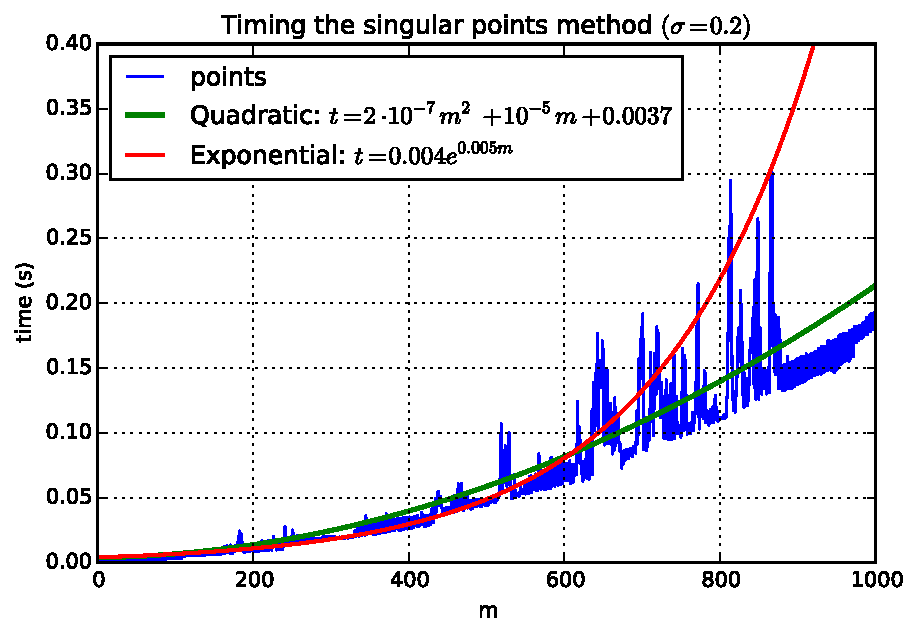
\includegraphics[width=\linewidth]{img/timing-cliquet}
	\caption[Timing -- cliquet]{Timing the singular point method for cliquet option with constant volatility $ \sigma = 0.2 $. The green line shows quadratic line fitted above most of the points, while the red line is the exponential in nature.}
	\label{fig:clq-timing}
\end{figure}


\begin{rem}[Computational complexity]
	We remarked earlier that although the computational complexity of the algorithm without approximation is the same as that of the binomial model, enabling approximations decreases the complexity to a polynomial time algorithm. In fact, the Figure \ref{fig:clq-timing} corroborates exactly to this. The blue dots denotes the time taken to run the algorithm for constant volatility of $ \sigma = 0.2 $. The green line is a quadratic function of the number of time steps $ m $, whereas the red line is an exponential function of the same. We varied the parameters so that the curves fits the data. We see that the quadratic function serves as an upper bound for the running time for most data points in the plot, except for a few points, which may be treated as outliers. Thus, we may conclude that the computational complexity of the algorithm is $ O(m^2) $ in this case. In fact, our experiments show that this is indeed the general trend. Thus, even though we have not found out the theoretical complexity of the algorithm, in practice the algorithm is competitive.
	
	Note that for the Asian case, the experimental complexity is $ O(n^3) $, whereas in the cliquet case, it is $ O(m^2) $.
\end{rem}


\paragraph{Concluding remarks}
We note that, in all cases, the difference between the prices in obtained by the singular points method and the binomial method is significantly smaller than the theoretical value of $ N \cdot 10^{-6} $. Moreover, as in the case examined $ N C_{loc} < C_{glob} $ (which is equivalent to $ N C_{loc} = C_{glob} $), the price functions $ V_i(Z) $ are always convex and this implies that the approximation procedure will provide an upper estimate of the exact binomial value.

Thus, the singular points method is quite capable in pricing cliquet options in a Black-Scholes framework with piecewise constant interest rates and volatilities. The implementation is quite simple, and the price obtained by the method converges to the price of continuous model. In absence of approximation, the price matches the exact binomial price. The ability to set \emph{a priori} error bounds differentiates it from the alternative algorithms.

Numerical comparisons indicate that the method is accurate both for standard and small volatilities, and that it avoids the computational problems arising from the application of the standard binomial method. For small volatilities and large numbers of observation times in particular, the improvement with respect to the binomial standard technique is very significant. Experimental results show that the computational complexity in practice is around $ O(m^2) $.


%%% Local Variables:
%%% LaTeX-command: "latex -shell-escape"
%%% mode: latex
%%% TeX-master: t
%%% End:
